\chapter{Практическая часть}
\label{cha:ch_2}

В рамках ВКР была реализована
библиотека hpfw (\href{https://github.com/kisasexypantera94/hpfw}{\color{blue} ссылка} на Github).
С использованием инструментов библиотеки была решена задача идентификации музыкальных
произведений по фрагментам концертных исполнений. Для этой же
задачи написан Telegram-бот (\href{https://t.me/hpfw_bot}{\color{blue} ссылка} на бота).

\section{Технологии}
В библиотеке hpfw используются:
\begin{itemize}
    \item C++17
    \item essentia -- для вычисления спектрограмм
    \item Eigen3 -- для линейной алгебры
    \item cpp-taskflow -- для распараллеливания индексации
\end{itemize}

Для библиотеки также написан Python-клиент.

\section{Архитектура библиотеки}
В центре библиотеки два класса -- $Collector$ (коллектор) и $HashprintHandle$ (хеншпринт-хендл).
Эти классы связаны паттерном <<Стратегия>>. Хендлы предоставляют инструменты (функции) для вычисления
хешпринтов. Коллекторы используют эти инструменты по своему усмотрению и занимаются непосредственно
вычислением хешпринтов. Благодаря такой структуре, можно будет легко тестировать различные способы
распараллеливания индексации.

$Collector$ хранит текущую аккумулированную ковариационную матрицу, фильтры и спектрограммы.
Таким образом чтобы добавить или удалить трек из базы достаточно:
\begin{enumerate}[label=\arabic*.]
    \item Посчитать ковариационную матрицу для матрицы фреймов трека и добавить/вычесть ее из
    аккумулированной ковариационной матрицы
    \item Пересчитать фильтры
    \item С использованием новых фильтров пересчитать хешпринты
\end{enumerate}
Самым узким местом индексации является именно вычисление спектрограмм. Храня их, мы в разы
ускоряем обновление базы.

\section{Клиент}
Пока что не очень ясно, где стоит проводить черту между библиотекой и клиентом. На данный момент
клиент использует только класс $Collector$, то есть хранилища и поиск реализуются уже на стороне клиента.
Самые узкие места поиска написаны на Cython.

\section{Telegram-бот}
Бот использует Python клиент.

Принцип работы:
\begin{enumerate}[label=\arabic*.]
    \item Пользователь записывает голосовое сообщение с отрывком трека. Также можно напеть или сыграть мелодию,
    но сделать это нужно в той же тональности и октаве.
    \item Бот с помощью API получает список событий. Если в событии есть голосовое сообщение,
    то он с помощью класса $Collector$ находит представление записи в виде хешпринтов, ищет
    совпадения в базе и возвращает пользователю топ-5 лучших совпадений.
\end{enumerate}
\begin{figure}[H]
    \centering
    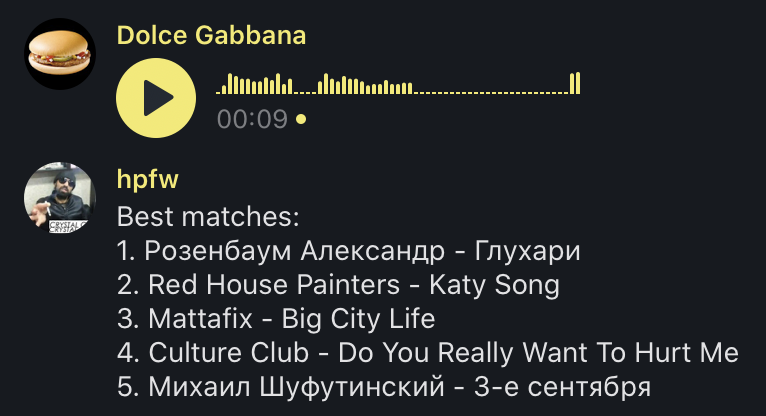
\includegraphics[scale=0.6]{inc/img/tgbot.png}
    \caption{Пример ответа на запрос пользователя}
\end{figure}

В планах внедрить механизм webhook.

\section{Результаты}
Замеры проводились на Intel i5-6360U (4) @ 2.00GHz, 8GB RAM
\begin{itemize}
    \item На индексацию одного трека уходит в среднем 5.7 секунд
    \item На полный поиск (без индекса) отрывка по базе из 167 треков уходит в среднем 300 миллисекунд
    \item Средняя по трекам точность поиска (без индекса) 216-ти 9-секундных отрывков по базе из 167 треков -- 0.9
    \item Одна спектрограмма занимает около 10 МБ (правда, их не всегда нужно хранить)
\end{itemize}

\subsection{Точность поиска в разрезе живых исполнений}
Поиск без индекса (полный перебор):
\begin{itemize}
    \item <<Буерак - На старых сидениях кинотеатра (live)>> -- 1.0 (24/24)
    \item <<The Smiths - There Is a Light That Never Goes Out (live)>> -- 1.0 (25/25)
    \item <<The Smiths - The Boy with the Thorn in His Side (live)>> -- 1.0 (22/22)
    \item <<The Killers - Mr. Brightside (live)>> -- 0.9583 (23/24)
    \item <<пасош - каждый день (live)>> -- 0.9545 (21/22)
    \item <<The Smiths - Cemetry Gates (live)>> -- 0.9333 (14/15)
    \item <<Joy Division - New Dawn Fades (live)>> -- 0.88 (22/25)
    \item <<Neil Young - Old Man (live)>> -- 0.8095 (17/21)
    \item <<The Doors - People Are Strange (live)>> -- 0.8 (12/15)
    \item <<Joy Division - Day Of The Lords (live)>> -- 0.7333 (22/30)
\end{itemize}

Поиск с предварительным отбором топ-30 кандидатов с помощью HNSW:
\begin{itemize}
    \item <<Буерак - На старых сидениях кинотеатра (live)>> -- 0.7916 (19/24)
    \item <<The Smiths - There Is a Light That Never Goes Out (live)>> -- 0.72 (18/25)
    \item <<The Smiths - The Boy with the Thorn in His Side (live)>> -- 1.0 (22/22)
    \item <<The Killers - Mr. Brightside (live)>> -- 0.6087 (15/24)
    \item <<пасош - каждый день (live)>> -- 0.619 (14/22)
    \item <<The Smiths - Cemetry Gates (live)>> -- 0.4285 (6/15)
    \item <<Joy Division - New Dawn Fades (live)>> -- 0.7826 (19/25)
    \item <<Neil Young - Old Man (live)>> -- 0.4285 (9/21)
    \item <<The Doors - People Are Strange (live)>> -- 0.7692 (11/15)
    \item <<Joy Division - Day Of The Lords (live)>> -- 0.3448 (10/30)
\end{itemize}

Можно заметить, что использование индекса по-разному влияет на каждый из треков.
На поиск подходящих параметров HNSW было потрачено довольно мало времени, так как
на данном этапе это попросту бесполезно -- преимущество HNSW будет ощутимо при наличии в базе
хотя бы 1000 треков.

Стоит отметить, что поиск осуществлялся без знания исполнителя, то есть это оценка в худшем случае.

\section{Дальнейшее развитие библиотеки}
\begin{enumerate}[label=\arabic*.]
    \item Оптимизация поиска -- исследовать другие алгоритмы поиска, сравнить их.
    \item Характеризация музыки. Многие современные рекомендательные системы используют
    коллаборативную фильтрацию, качество которой практически полностью зависит от пользователей.
    Рекомендации, построенные на методе хешпринтов будут лишены недостатков
    коллаборативной фильтрации.
    \item Попробовать решить задачи, традиционно решаемые с помощью нейросетей.
    Рассмотренный метод применим не только к аудиофайлам, но также к любым данным, представленным
    в виде временных рядов.
    Пандемия COVID-19 показала неготовность человечества к столкновению со слабо исследованными
    болезнями. Возможно наличие такого гибкого инструмента, способного работать на неразмеченных данных,
    сможет помочь.
    \item Распознавание трека по напеванию.
\end{enumerate}